\documentclass[12pt]{beamer}

\usepackage{tikz}
\usepackage{graphicx}
\usepackage[T1]{fontenc}
\usepackage{amsmath}
\usepackage{multicol}
\usepackage{booktabs, braket} % For formal tables
\usepackage{cleveref}
\usepackage{graphicx}
\usepackage{blkarray}
\usetikzlibrary{graphs, graphs.standard}

\DeclareMathOperator{\E}{\textrm{E}}		     % expected value
\DeclareMathOperator{\pr}{\mathrm{P}}		     % probability 
\DeclareMathOperator{\cov}{t_{cov}}	             % cover time

\DeclareMathOperator{\X}{\mathbb{X}}		     % expected value
\DeclareMathOperator{\tr}{\text{tr}}		     % trace
\DeclareMathOperator{\Ap}{$A$ ^\prime} 		     % A'
\DeclareMathOperator{\bp}{$b$ ^\prime} 		     % b'
\DeclareMathOperator{\Xb}{\mathcal{X}}		     % big X

\title{Semidefinite Programming and Quantum Algorithms}
\author{Michael Czekanski \& R. Teal Witter}
\institute{Middlebury College}
\date{November 5, 2019}

\begin{document}
\graphicspath{{./../figures/}}

\frame{\titlepage}

\begin{frame}{Overview}
\tableofcontents
\end{frame}

\section{Query Complexity}
\begin{frame}{Query Complexity}
\begin{center}
The number of times an algorithm queries the input.
\end{center}
\begin{table}[]
\begin{tabular}{cc}
\hline
\textbf{Input} & \textbf{Output} \\ \hline
00             & 0               \\
01             & 1               \\
10             & 1               \\
11             & 1               \\ \hline
\end{tabular}
\end{table}
\end{frame}

\section{Semidefinite Programming}

\begin{frame}{Quantum Query Complexity as SDP: Reichardt \cite{reichardt2009span}}
\begin{align} \label{eq:reichardtObj} 
    f_{\text{bound}} = \min_{\X} M(\X) = \max_{y \in D} \sum_{j \in [n]}
    \bra{y,j}\X\ket{y,j} 
\end{align}
Subject to
\begin{align}\label{Eq:reichardtSemi}
    \X \succcurlyeq 0 
\end{align}
\begin{align}\label{Eq:reichardtOffDiag}
    \forall (y,z) \in F \sum_{j \in [n]: y_j \ne z_j} 
    \bra{y,j} \X \ket{z, j} = 1.
\end{align}
\end{frame}

\begin{frame}{A Standard Form: Boyd\cite{boyd2004convex}}
Minimize
\begin{align}\label{Eq:boyd_obj}
    M(\X) = \tr(C\X) 
\end{align}
Subject to
\begin{align} \label{Eq:boydSemi}
    \X \succcurlyeq 0   
\end{align}

\begin{align} \label{Eq:boydTraceCon}
    \tr(A_i \X) = b_i  \text{$\qquad$ for $i \in \{1,...,p\}$}
\end{align}
\end{frame}

\section{Alternating Direction Methods}
\begin{frame}{We use ADM \cite{adm}}
\centering
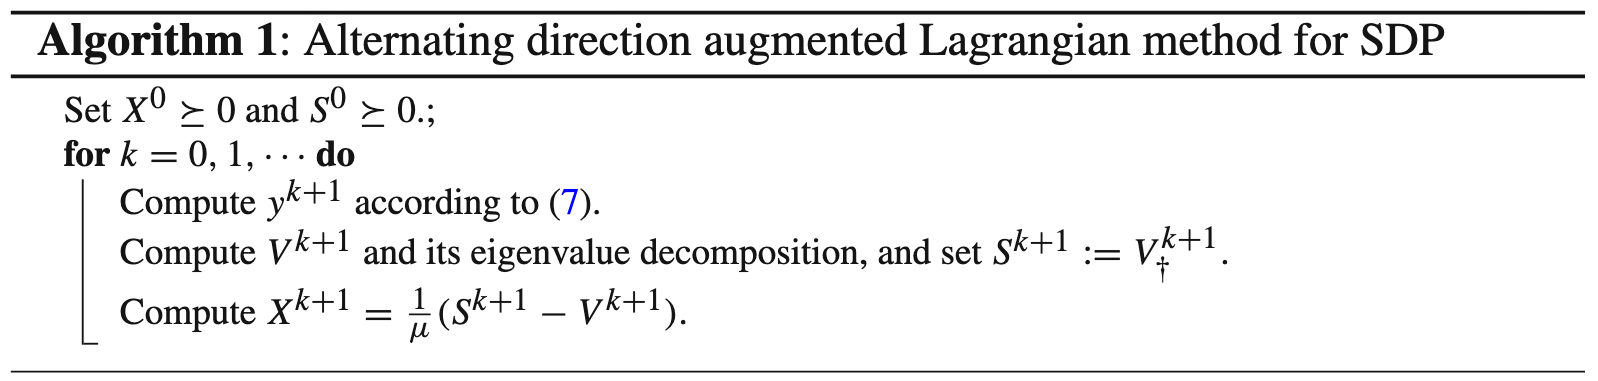
\includegraphics[scale=.15]{figures/adm_algorithm}
\bigskip
\begin{itemize}
    \item Easy to implement
    \item Exploits sparsity (yay zeroes!)
    \item Exploits constraint orthogonality
\end{itemize}
\end{frame}

\section{Our Work}
\begin{frame}{Numerial Results: Our Algorithm is Good.}
\centering
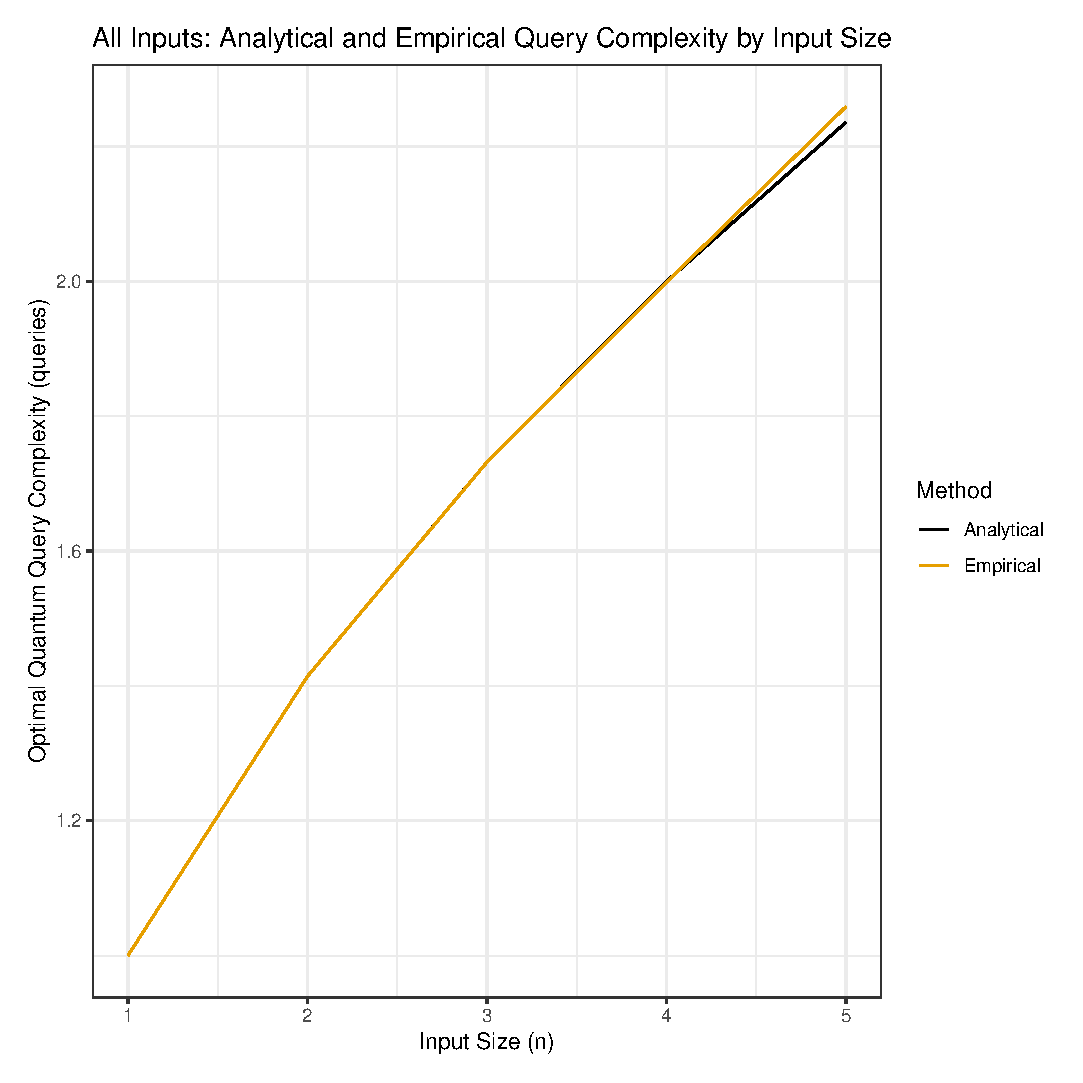
\includegraphics[scale=.5]{figure_all_or_complexity.eps}
\end{frame}

\begin{frame}{Run Time Results: Our Algorithm is Bad.}
\centering
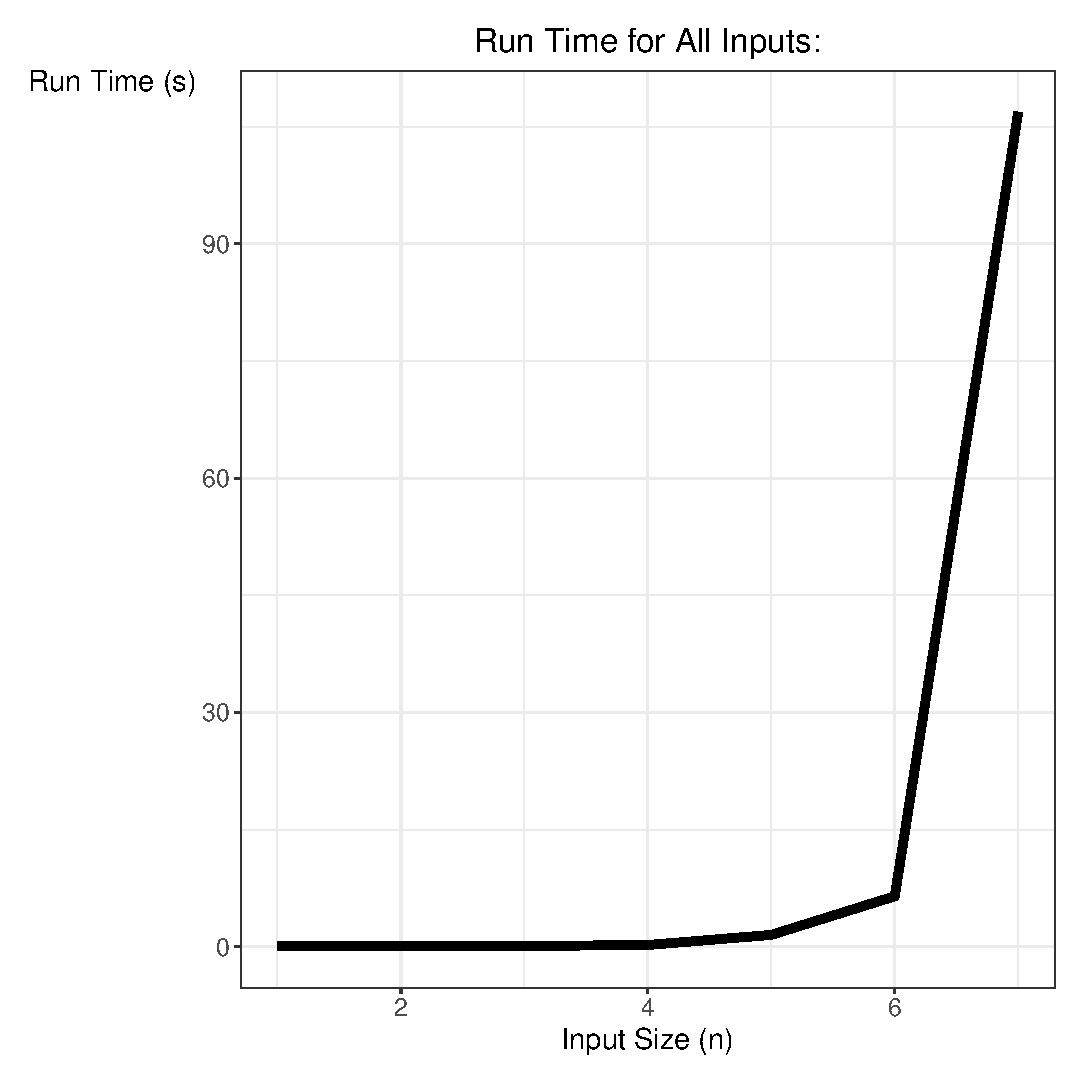
\includegraphics[scale=.5]{figure_all_or_time.eps}
\end{frame}

\begin{frame}{We Have Plans (For the Future)}
\begin{itemize}
    \item Document
    \item More optimization
    \item Span program
\end{itemize} 
\end{frame}

\begin{frame}{Thank you!}
\bibliographystyle{abbrv}
\bibliography{main}
\end{frame}

\end{document}